\tableofcontents
\pagebreak

\section{Свободное движение}
Рассмотрим систему второго порядка в форме В-В:
\begin{equation}
    \ddot{y} + a_1 \dot{y} + a_0 y  = u
\end{equation}
Согласно заданию, выберем три набора корней $(\lambda_1, \lambda_2)$, удовлетворяющих модам из задания (2,3,8)
и найдем небходимы пары коэффициентов $(a_1, a_0)$:
\begin{enumerate}
    \item Нейтральная и устойчивая апериодическая: $\lambda_1 = 0, \lambda_2 = -1$; $a_1 = 1, a_0 = 0$
    \item Нейтральная и неустойчивая апериодическая: $\lambda_1 = 0, \lambda_2 = 0.3$; $a_1 = -0.3, a_0 = 0$
    \item Пара неусточивых колебательных мод: $\lambda_1 = 0.4 + 2i, \lambda_2 = 0.4 - 2i$; $a_1 = -0.8, a_0 = 4.16$
\end{enumerate}


\begin{figure}[h]
    \centering
    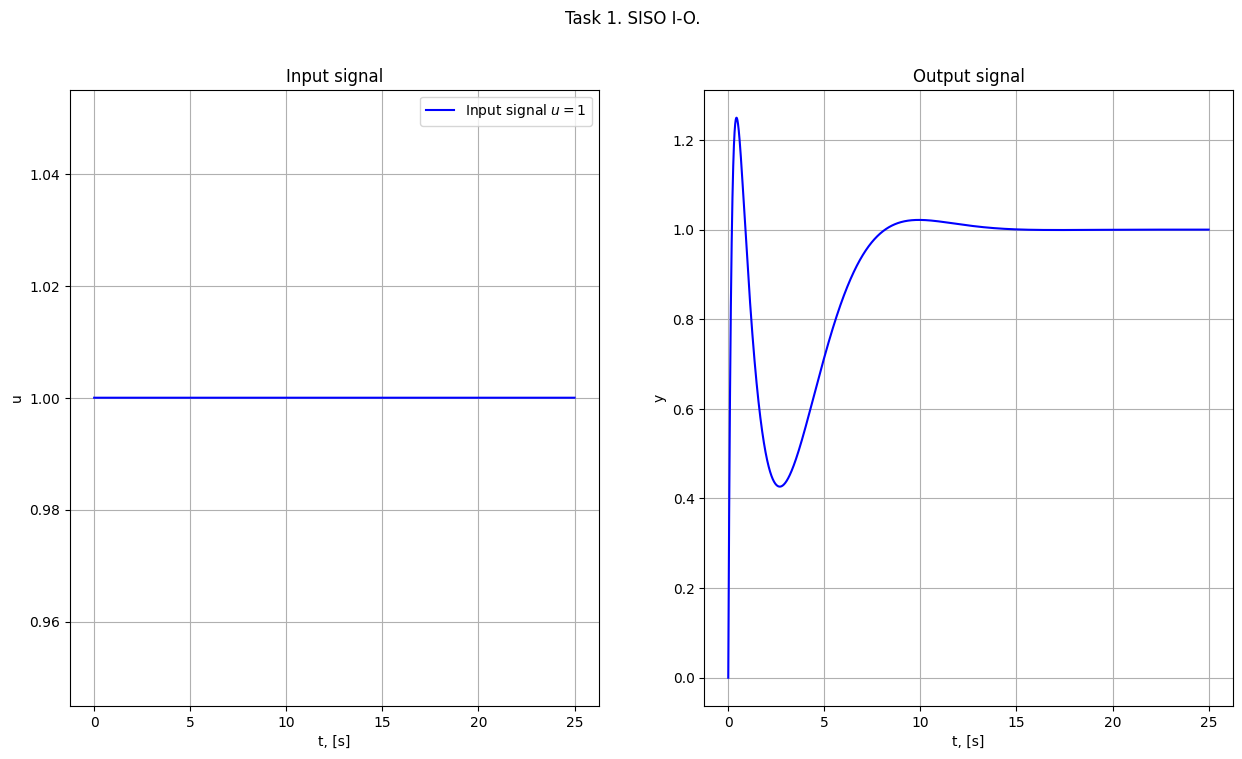
\includegraphics[width=\textwidth]{plot_1_1}
    \caption{\label{fig:The-caption-1}Входные и выходные сигналы систем при нулевых начальных условиях (задание 1)}
\end{figure}

Вычисления пары $(a_1, a_0)$ проведем, воспользовавшись теоремой Виета:
\begin{equation*}
    \begin{cases}
        \lambda_1 + \lambda_2 = - a_1 \\
        \lambda_1 \lambda_2 = a_0
    \end{cases}
\end{equation*}
Согласно корневому критерию, первый набор корней соответствует апериодической системе на границе 
 устойчивости (оба корня действительные, неотрицательны и не кратные), второй - неустойчивой 
 апериодической системе (корни действительные, один из корней имеет положительную действительную часть),
 третий - неустойчивой колебательной системе (пара комплексно сопряженных корней с положительной 
 действительной частью).

 Проведем моделирование поведения систем с нулевыми начальными условиями и при $y(0)=0, \dot y (0) = 1$ 
 (рис. 1 и рис. 2 соответственно).
 

 \begin{figure}[h]
    \centering
    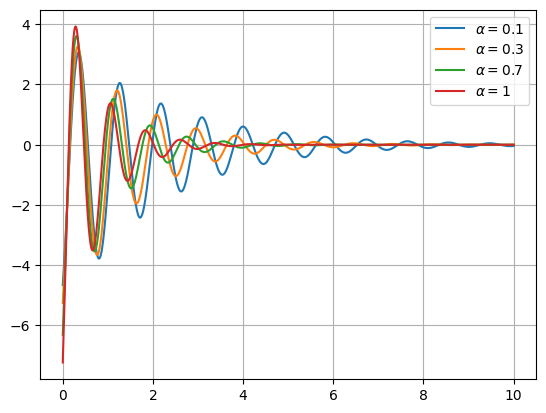
\includegraphics[width=\textwidth]{plot_1_2}
    \caption{\label{fig:The-caption-1}Входные и выходные сигналы систем при ненулевых начальных условиях (задание 1)}
\end{figure}

Заметим, что все системы ведут себя одинаково при задании нулевых начальных условий 
и подаче нулевого управляющего воздействия (они статичны в 0). При задании начальных условий системы
ведут себя согласно аналитически предсказанному корневым критерием.

\pagebreak

\section{Область устойчивости}

\pagebreak

\section{Автономный генератор}

\pagebreak

\section{Изучение канонической управляемой формы: фазовые портреты}

\pagebreak